\documentclass[../../main.tex]{subfiles}

\begin{document}
    
    \section{Steganalysis}
    Steganalysis is the branch os study dedicated at analysing the methods and the vectors used to transmit an hidden message in order to retrieve such message whenever it is present.
    Unlike chryptanalysis where the message may even be apparent but enchrypted, in steganalysis the study of the message starts from a suspect.
    \subsection{Methods}
    Hereinafter we will present the two type of methods used in steganalysis in order to obtain the secret message 

    \subsubsection{Statistical}

    \subsubsection{Structural}
    

    \subsection{Cover Types}

    \subsubsection{Images}


    \subsubsection{Audio}
    
    
    \subsubsection{Text}
    
    
    \subsubsection{TCP/IP}
    Before treating such topic we must briefly discuss the behaviour of the TCP/IP (\textbf{Internet protocol suit}) communications.
    
    \textbf{IP (Internet Protocol)} is at the basis of internet communication. The protocol exploits the principle of encapsulation, sending packets composed by a \emph{header} which contains information such as the \textbf{destination address} and \textbf{source address} and a \emph{payload}
    which represents the actual data to be transmitted. Since physical channels usually have a limited \emph{MTU}\footnote{Maximum Transmission Unit}, then the data is usually fragmented in smaller chunks, wrapped into an header and only then transmitted.
    
    \textbf{TCP (Transmission Control protocol)} is a protocol used for reliable(little information loss), ordered, error-checked data transmission between a machine
    hosting the data (\textbf{Server}) and another requiring such data (\textbf{Client}). It is performed previous a three-way handshake which estabilishes a connection between server and client, thus preparing 
    a reliable communication channel.
    \begin{figure}[h]
        \centering
        \caption{Structure of TCP packet}
        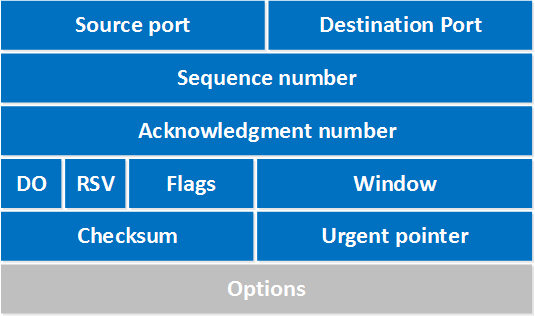
\includegraphics[scale=0.5]{tcp_header.png}
    \end{figure}
    \pagebreak

    \textbf{UDP (User Datagram Protocol)}, contrary to TCP, is less reliable but faster.
     It broadcasts the data in an unordered and uncontrolled way to the receiver. 
    There is no need to estabilishing a connection in order to implement such protocol.

    \begin{figure}[h]
        \centering
        \caption{Structure of TCP packet}
        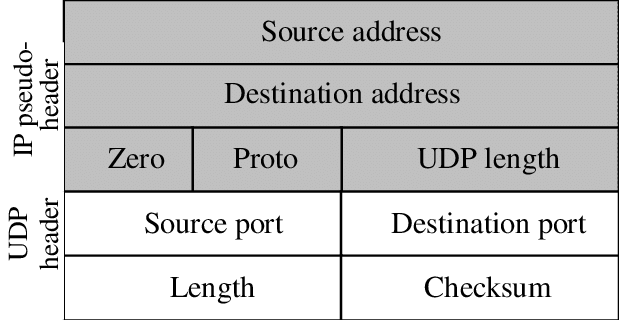
\includegraphics[scale=0.3]{udp_header.png}
    \end{figure}

    As you could notice from the previous figures, the first part of the header is the same. This is because it is part of the IP protocol itself.
    In the second part of each header we find different types of metadata which are specific for each protocol. Generally the metadat contained in the header is redundant 
    for the transmission of the message itself and this redundancy may become a target for a \emph{stego-algorithm}\footnote{an algorithm used for steganography} which starting from a 
    \emph{cover-network packet sequence}\footnote{a sequence of packets which will be transmitted over the network acting as a cover for the hidden messace} and a \emph{covert message}, can generate a sequence of packets(each one embedding a portion of the covered message) which will be sent over the network.

    This procedure is not a \emph{risk-free} approach for the attacker who wishes to send the \emph{cover-network packet sequence}, since it is possible that the data will be currupted during transmission or there could be losses using non-reliable transport protocols(UDP).
    Other criticalities of such method stay in the fact that the sequence of packets will most likely traverse multiple nodes in the network before reaching the target, and the message may be detected by these nodes.

    


    \pagebreak
\end{document}